\vspace{-0.2cm}
\section{Final Results}
\label{sec:results}

\looseness -1 We now present evaluations of our model, \ourmodel 8B. To avoid making decisions based on future information, we evaluate on test sets that were not observed until the end.\vspace{0.15cm}

\textbf{Open-ended Test Set.} Given the lack of \emph{open-ended} forecasting benchmarks that are still ``in the future'' for our models, we create our own test set with additional steps to ensure high quality. We first use our data creation recipe to generate an initial set of 1,000 questions between May to August 2025 using a stronger model, \texttt{o4-mini-high}. We draw from five diverse news sources: Al Jazeera English (global news, based out of Qatar), Time (global news, based out of USA) The Independent (UK focused), Fox News (USA focused), NDTV (India focused), with 200 questions selected from each. The choice of sources was made under the constraint of many established news sources have disallowed crawling of their articles starting 2025.
We deliberately use distinct sources from the training set to ensure that our model is learning generalizable forecasting skills, and not source distribution specific biases. Beginning from this initial set of 1000 questions, we perform additional filtering steps to prepare a high-quality test set: 
\begin{enumerate}
    \item We remove any potentially unanswerable questions (noise) by keeping only those which \texttt{grok-4.1-fast} could successfully answer with search tool access ($85\%$).
    \item To address the issue of late reporting in news outlets, we again use \texttt{grok-4.1-fast} with search tool to find the \textbf{earliest resolution date} for a given question. This is important to prevent leakage from retrieving articles with the true answer. We retain only those questions with resolution date after May 2025 ($64\%$).
    \item Finally, we manually filter the remaining questions to meet our quality checks, resulting in a final test set of $302$ questions. We provide more details like news source specific statistics in \Cref{sec:test_set_details}.
\end{enumerate} 

\textbf{External Datasets.} We use the FutureX benchmark~\citep{zeng2025futurex}, filtering to non-numeric, English, resolved forecasting questions and evaluating all models with our retrieval. This leaves 86 binary or multiple choice questions, between July to August 2025. For evaluating long-term predictions (without retrieval), we measure consistency metrics on binary questions up to 2028 as proposed by ~\citet{paleka2025consistency}, who show they correlate strongly with forecasting performance. Finally, to measure whether our forecasting training generalizes to calibration on standard benchmarks of LLM capabilities, we evaluate without retrieval on a challenging factuality benchmark, SimpleQA \citep{wei2024measuringshortformfactualitylarge}, and popular cross-domain reasoning benchmarks, MMLU-Pro and GPQA-Diamond. \vspace{0.15cm}

\begin{figure}[t]
\vspace{-0.25cm}
    \centering
    % Legend
    
\includegraphics[width=0.9\linewidth]{figures/testset-final/scatter_brier_accuracy_test5news_302_Llama_4_Scout_legend.pdf}
    \hfill

    % (a) left plot
    \begin{subfigure}[t]{0.49\textwidth}
        \centering
        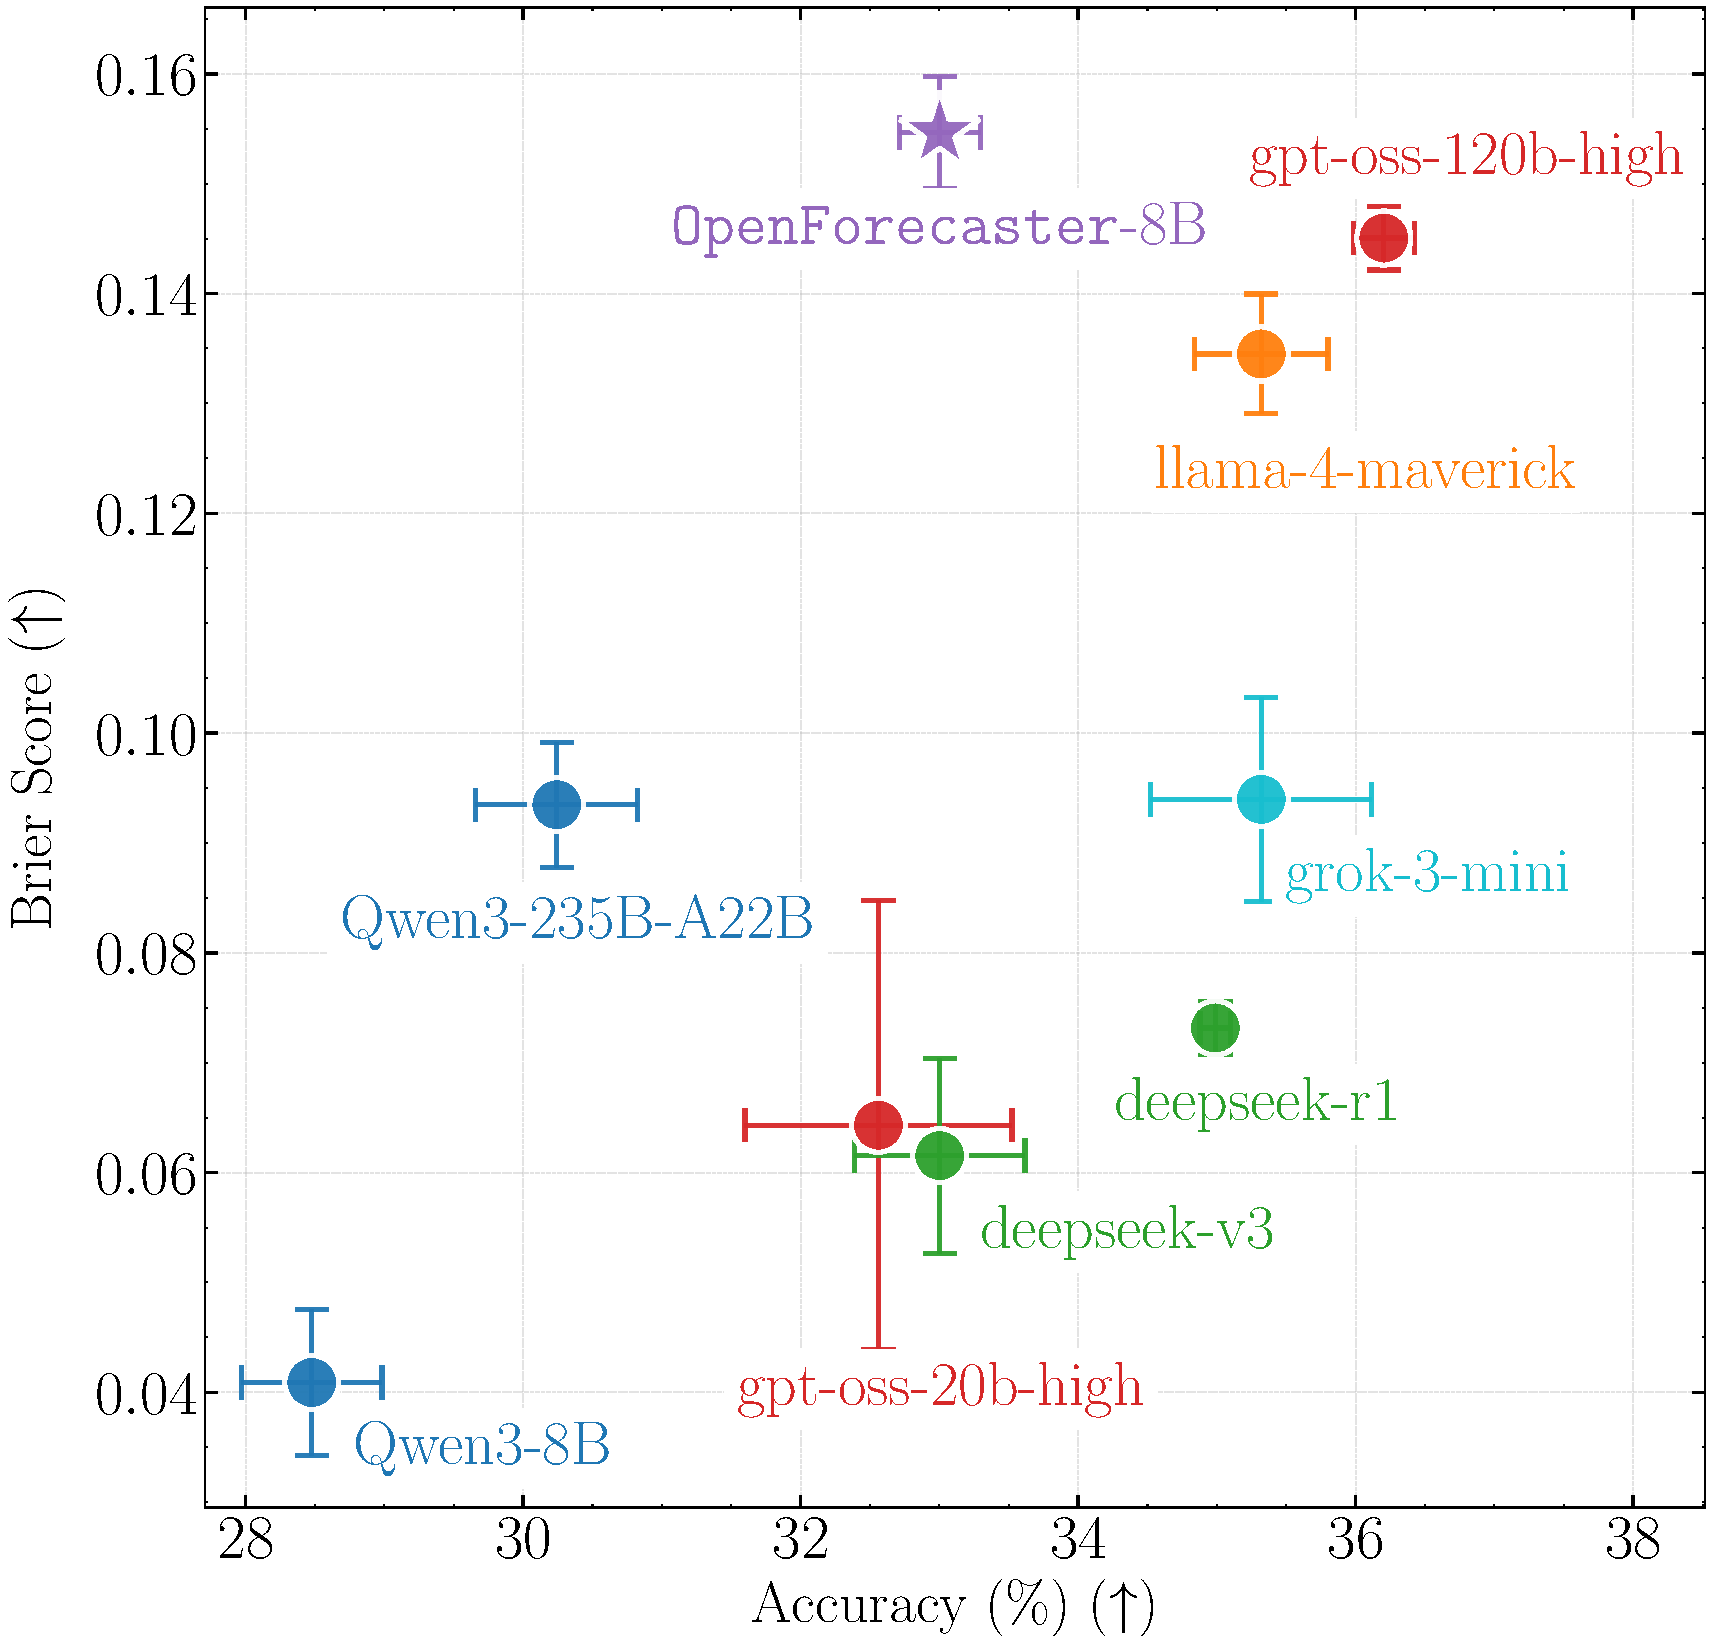
\includegraphics[width=0.9\linewidth]{figures/testset-final/scatter_accuracy_brier_test5news_302_Llama_4_Scout.pdf}
        \caption{Results on \ourdataset\; May-Aug 2025.}
        \label{fig:test_set_performance}
    \end{subfigure}
    \hfill
    % (b) right plot
    \begin{subfigure}[t]{0.49\textwidth}
        \centering
        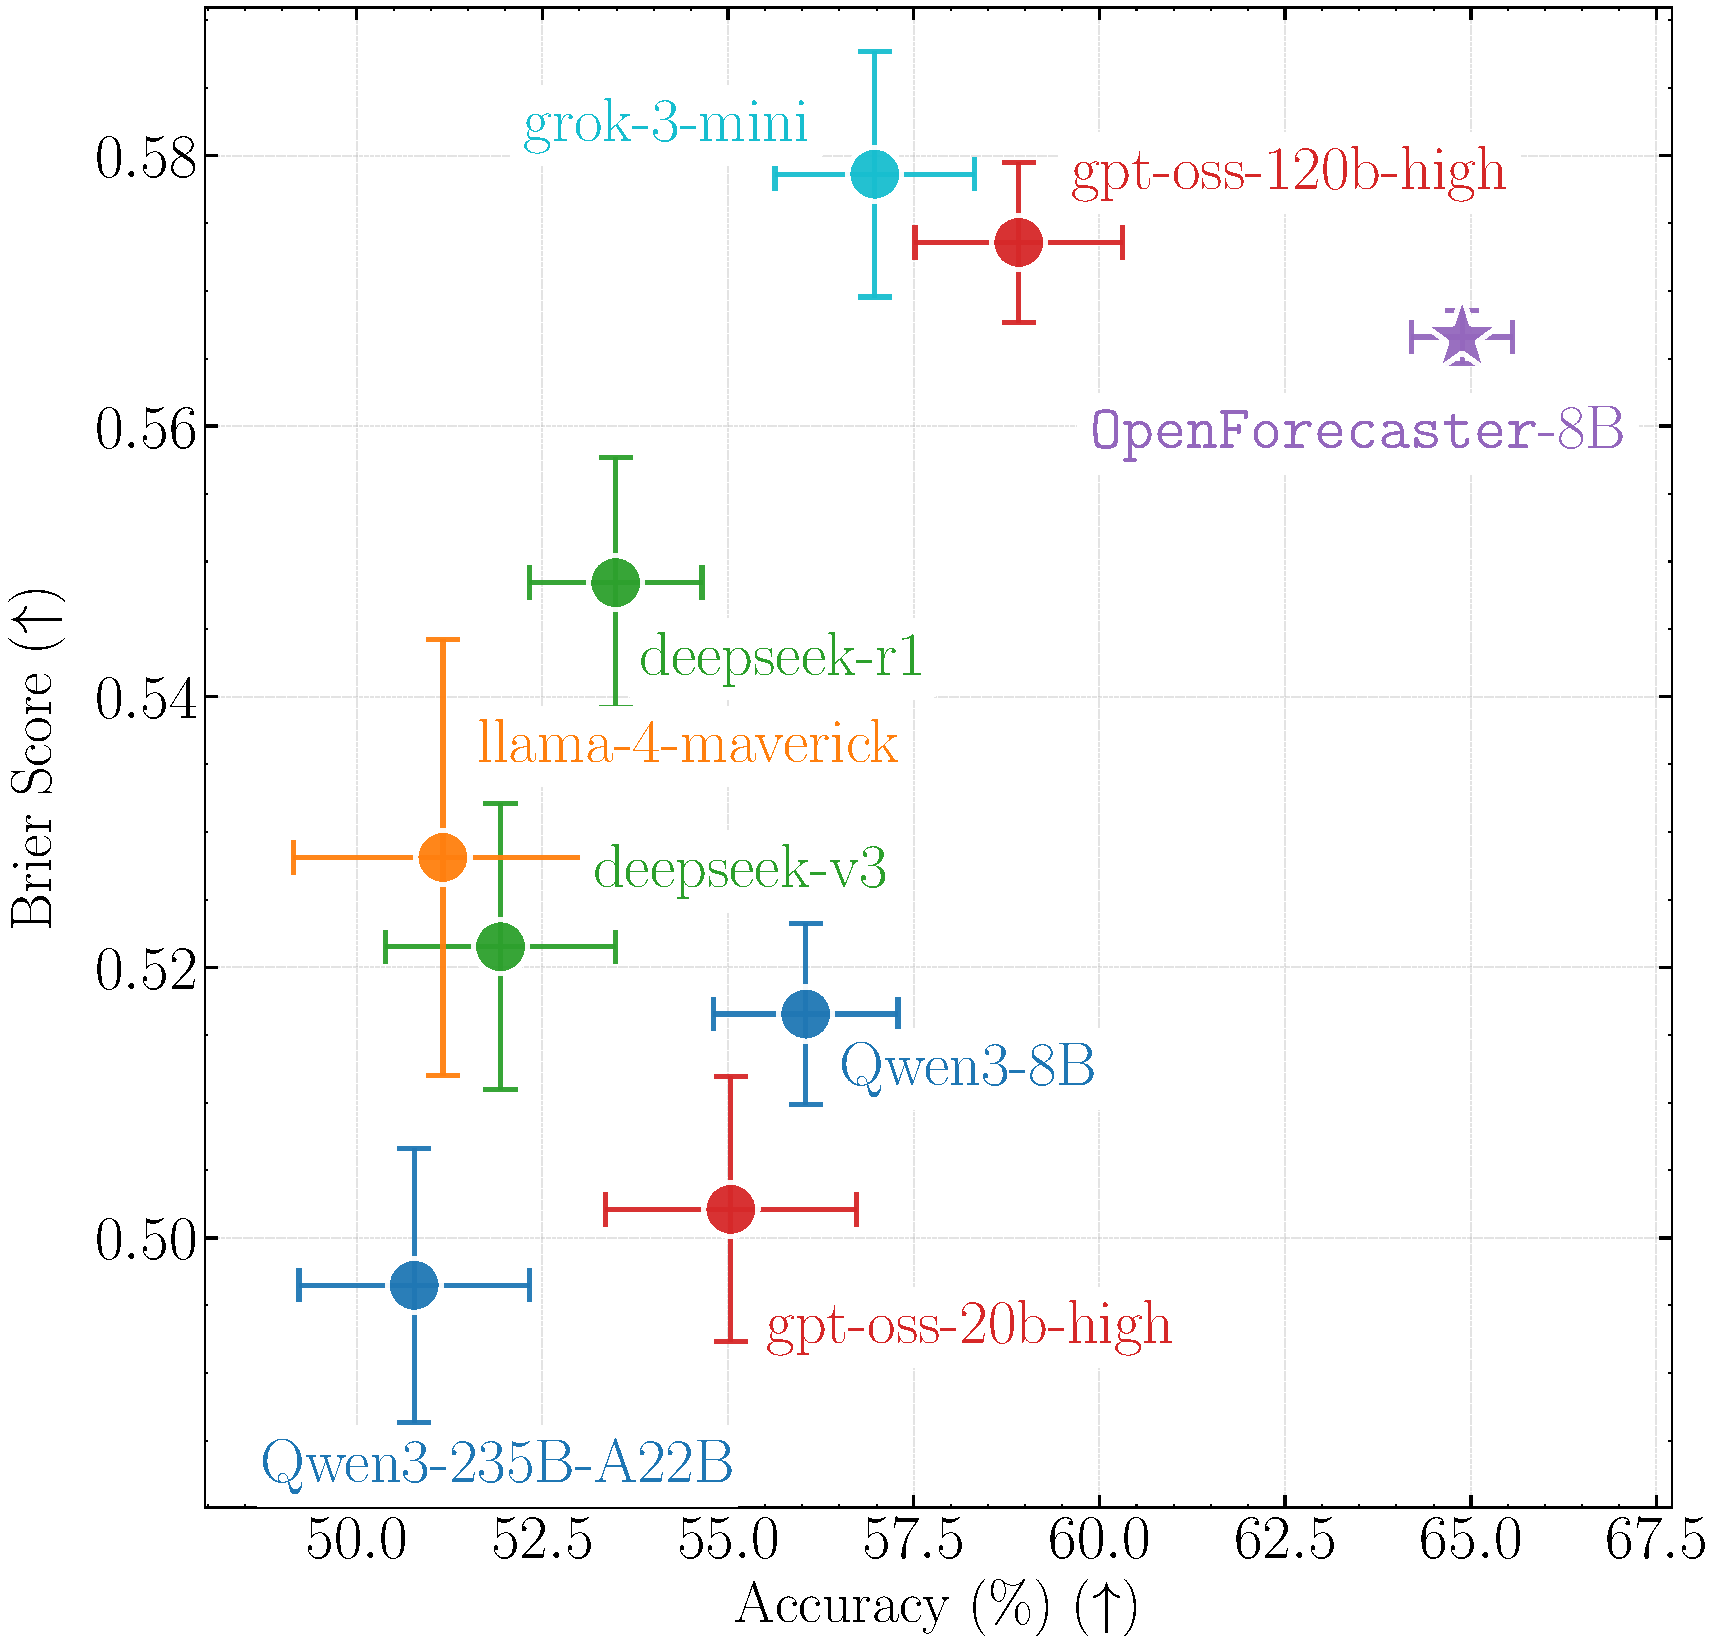
\includegraphics[width=0.9\linewidth]{figures/futurex/scatter_accuracy_brier_futurex-past86-retrieval.pdf}
        \caption{ 
            Results on FutureX July-Aug 2025.
             }
        \label{fig:futurex_performance}
    \end{subfigure}

    \caption{
        \textbf{Our forecasting training improves accuracy and calibration} both on open-ended questions in our test set,  and the external FutureX benchmark. It makes \ourmodel 8B competitive with much larger models that have knowledge cutoffs before May 2025.  
    }
    \vspace{-.2cm}
\end{figure}

\begin{figure}[h]
\vspace{-0.0cm}
    \centering
   
    % (a) left plot
    \begin{subfigure}[t]{0.49\textwidth}
        \centering
        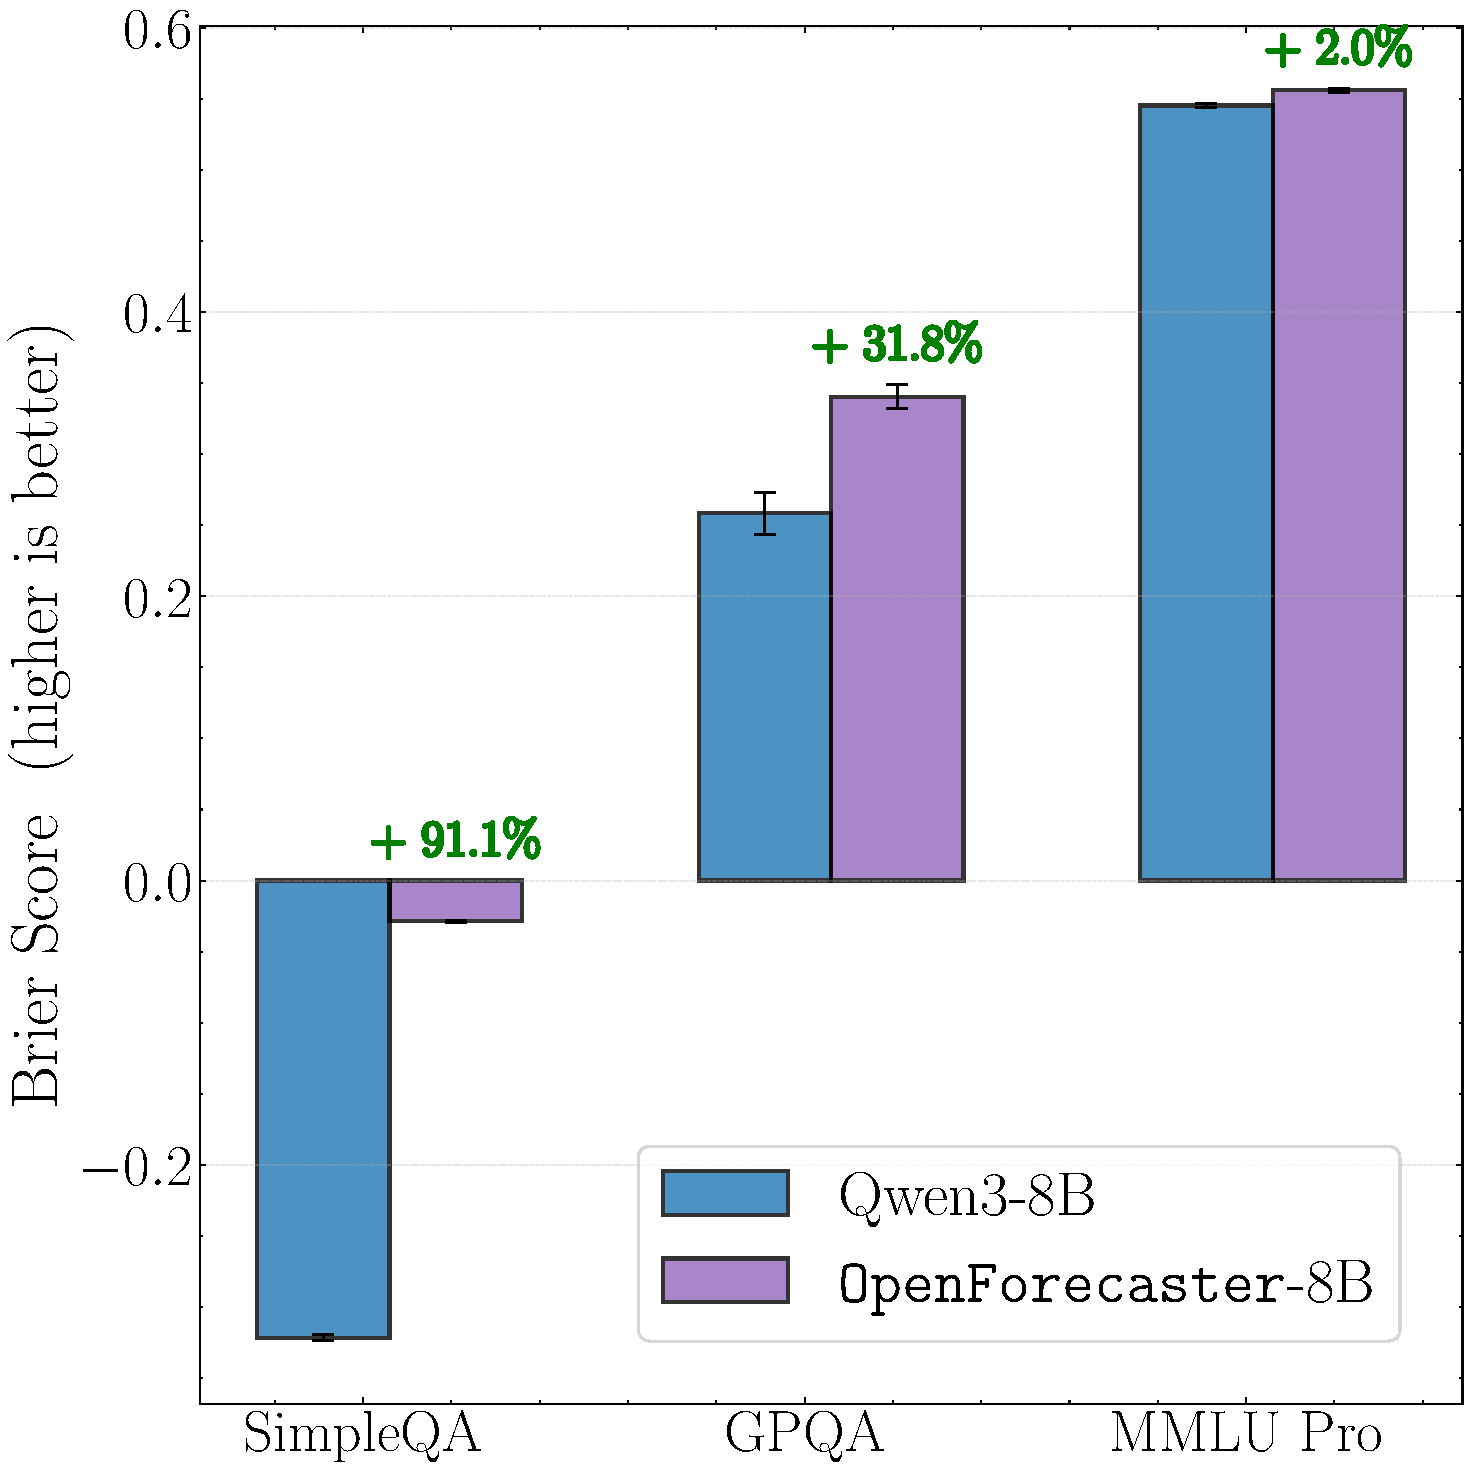
\includegraphics[width=0.95\linewidth]{figures/otherbenchmarks/brier_comparison.pdf}
        \caption{Brier score on general benchmarks.}
        \label{fig:simpleqa_performance}
    \end{subfigure}
    \hfill
    % (b) right plot
    \begin{subfigure}[t]{0.49\textwidth}
        \centering
        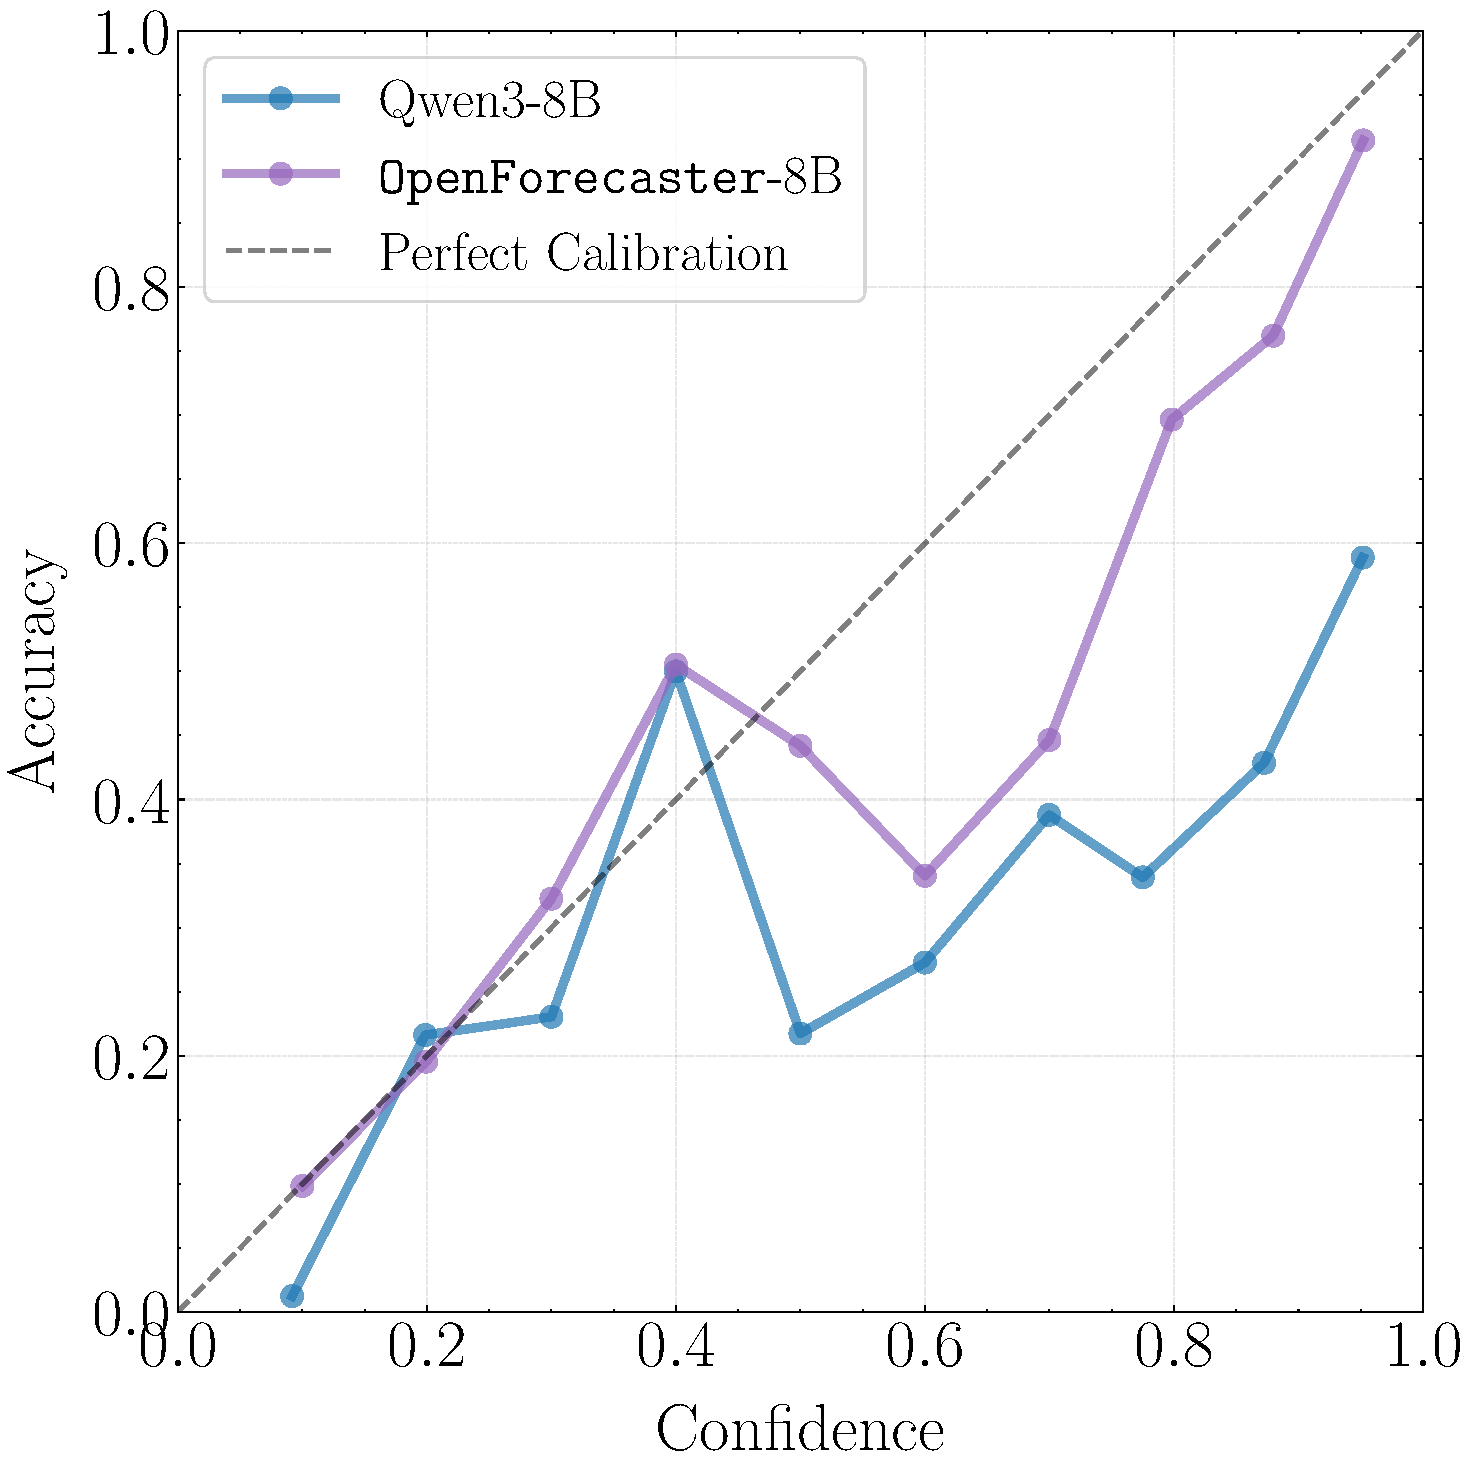
\includegraphics[width=0.95\linewidth]{figures/testset-final/calibration_curves_8B.pdf}
        \caption{Calibration curve on our test set. }
        \label{fig:calibration_curve}
    \end{subfigure}
\vspace{-.2cm}
    \caption{Calibration of the models improve significantly after training on \ourdataset \ both on (a) out of distribution benchmarks and (b) on \ourdataset \ test set.}
    
    \vspace{-.25cm}
\end{figure}

\contribution{Result 4: Training on our dataset leads to large improvements in forecasting.}
\Cref{fig:test_set_performance} shows performance of models on our held-out test set of open-ended forecasting questions. On the Brier score (Y axis), the primary metric recommended for forecasting~\citep{tetlock2016superforecasting}, as it measures both accuracy and calibration, \ourmodel 8B outperforms even GPT OSS 120B. Our improvements are not merely from calibration, the predictions also become more accurate (X axis), beating Qwen3 235B, but are a bit behind others. Training on \ourdataset \ also improves models from other families like Llama and Gemma as we show in \Cref{sec:extra_forecasting_results}. We saw a particularly large (+25\% absolute improvement in accuracy) improvement for Llama 3.1 8B Instruct, surpassing the much larger Qwen3-235-A22B. We also show model accuracy by month in ~\Cref{fig:monthly_accuracy}. \vspace{0.15cm}

\looseness -1 On FutureX, our model has the strongest accuracy by a large margin, even compared to much larger proprietary counterparts. It is close to the best for Brier score as well. Finally, our training leads to more consistent long-term predictions, improving 44\% on arbitrage metrics, and 19\% on frequentist metrics, with detailed results in \Cref{sec:consistency}. Our model also improves on questions from Metaculus prediction market albeit staying behind few larger models which we show in \Cref{sec:metaculus_results}.

% \textbf{Improvements on External Forecasting Benchmark.}
% We also validate our models on resolved questions from the %established 
% existing FutureX \citep{zeng2025futurex} dataset\footnote{\url{https://huggingface.co/datasets/futurex-ai/Futurex-Past}}. We filter to English and non-numeric questions, which leaves only 86 binary or multiple choice samples. In \Cref{fig:futurex_performance}, we plot the performance of the models. Training on \ourdataset \ leads to large performance improvements, making our 8B model outperform GPT-OSS-120B. \vspace{0.15cm}

\contribution{Result 5: Calibration training for forecasting generalizes to other domains.} \Cref{fig:simpleqa_performance} shows downstream improvements in calibration across SimpleQA, GPQA-Diamond and MMLU-Pro (green text highlighting the relative improvement).
This calibration can then be used to reduce hallucinations, for example abstaining on questions the model is not confident about, using simple rules like \texttt{if probability < 0.1, replace prediction with ``I do not know''}\vspace{0.15cm}

% \textbf{Summary.} RL training on \texttt{OpenForesight} with our proposed reward for forecasting delivers large gains in both Brier score and accuracy, making small specialized models competitive with large general ones like DeepSeek R1 and gpt-oss-120B. Improvements in calibration generalize to out of distribution benchmarks.